\documentclass[
10pt, % Main document font size
a4paper, % Paper type, use 'letterpaper' for US Letter paper
oneside, % One page layout (no page indentation)
%twoside, % Two page layout (page indentation for binding and different headers)
headinclude,footinclude, % Extra spacing for the header and footer
BCOR5mm, % Binding correction
]{scrartcl}

\usepackage{amsmath,amssymb,amsfonts}
\usepackage{latexsym}
\usepackage{graphicx}
\usepackage{verbatim}
\usepackage{booktabs}
\usepackage[usenames,dvipsnames,svgnames,table]{xcolor}
\usepackage[framed,numbered,autolinebreaks,useliterate,final]{mcode}
\usepackage{listings}
\usepackage{multirow}
\usepackage{sectsty}

%%%%%%%%%%%%%%%%%%%%%%%%%%%%%%%%%%%%%%%%%
% Arsclassica Article
% Structure Specification File
%
% This file has been downloaded from:
% http://www.LaTeXTemplates.com
%
% Original author:
% Lorenzo Pantieri (http://www.lorenzopantieri.net) with extensive modifications by:
% Vel (vel@latextemplates.com)
%
% License:
% CC BY-NC-SA 3.0 (http://creativecommons.org/licenses/by-nc-sa/3.0/)
%
%%%%%%%%%%%%%%%%%%%%%%%%%%%%%%%%%%%%%%%%%

%----------------------------------------------------------------------------------------
%	REQUIRED PACKAGES
%----------------------------------------------------------------------------------------

\usepackage[
nochapters, % Turn off chapters since this is an article
beramono, % Use the Bera Mono font for monospaced text (\texttt)
eulermath,% Use the Euler font for mathematics
pdfspacing, % Makes use of pdftex�� letter spacing capabilities via the microtype package
dottedtoc % Dotted lines leading to the page numbers in the table of contents
]{classicthesis} % The layout is based on the Classic Thesis style

\usepackage{arsclassica} % Modifies the Classic Thesis package

\usepackage[T1]{fontenc} % Use 8-bit encoding that has 256 glyphs

\usepackage[utf8]{inputenc} % Required for including letters with accents

\usepackage{graphicx} % Required for including images
\graphicspath{{Figures/}} % Set the default folder for images

\usepackage{enumitem} % Required for manipulating the whitespace between and within lists

\usepackage{lipsum} % Used for inserting dummy 'Lorem ipsum' text into the template

\usepackage{subfig} % Required for creating figures with multiple parts (subfigures)

\usepackage{amsmath,amssymb,amsthm} % For including math equations, theorems, symbols, etc

\usepackage{varioref} % More descriptive referencing

%----------------------------------------------------------------------------------------
%	THEOREM STYLES
%---------------------------------------------------------------------------------------

\theoremstyle{definition} % Define theorem styles here based on the definition style (used for definitions and examples)
\newtheorem{definition}{Definition}

\theoremstyle{plain} % Define theorem styles here based on the plain style (used for theorems, lemmas, propositions)
\newtheorem{theorem}{Theorem}

\theoremstyle{remark} % Define theorem styles here based on the remark style (used for remarks and notes)

%----------------------------------------------------------------------------------------
%	HYPERLINKS
%---------------------------------------------------------------------------------------

\hypersetup{
%draft, % Uncomment to remove all links (useful for printing in black and white)
colorlinks=true, breaklinks=true, bookmarks=true,bookmarksnumbered,
urlcolor=webbrown, linkcolor=RoyalBlue, citecolor=webgreen, % Link colors
pdftitle={}, % PDF title
pdfauthor={\textcopyright}, % PDF Author
pdfsubject={}, % PDF Subject
pdfkeywords={}, % PDF Keywords
pdfcreator={pdfLaTeX}, % PDF Creator
pdfproducer={LaTeX with hyperref and ClassicThesis} % PDF producer
} % Include the structure.tex file which specified the document structure and layout

%\usepackage{times}
%\usepackage[mtbold,mtpluscal,mtplusscr]{mathtime}
%\usepackage{mathptmx}
\hyphenation{Fortran hy-phen-ation} % Specify custom hyphenation points in words with dashes where you would like hyphenation to occur, or alternatively, don't put any dashes in a word to stop hyphenation altogether
\theoremstyle{definition}
\newtheorem{thm}{Theorem}
\newtheorem{defn}[thm]{Definition}
\newtheorem{lem}{Lemma}[thm]
\newtheorem{cor}{Corollary}[thm]
\newtheorem{prop}{Proposition}[thm]
\newtheorem{rem}{Remark}[thm]
\newtheorem{ill}{Illustration}[thm]
%----------------------------------------------------------------------------------------
%	TITLE AND AUTHOR(S)
%----------------------------------------------------------------------------------------

\title{\normalfont\spacedallcaps{Numerical Analysis Project \#2 }} % The article title
\author{}
\date{}
\author{\spacedlowsmallcaps{Xinglu Wang}
\\  Student Number: 3140102282
\\ \vspace{0.5em}College of Information Science \& Electronic Engineering} % The article author(s) - author affiliations need to be specified in the AUTHOR AFFILIATIONS block

\date{} % An optional date to appear under the author(s)

%----------------------------------------------------------------------------------------

\begin{document}

%----------------------------------------------------------------------------------------
%	HEADERS
%----------------------------------------------------------------------------------------

\renewcommand{\sectionmark}[1]{\markright{\spacedlowsmallcaps{#1}}} % The header for all pages (oneside) or for even pages (twoside)
%\renewcommand{\subsectionmark}[1]{\markright{\thesubsection~#1}} % Uncomment when using the twoside option - this modifies the header on odd pages
\lehead{\mbox{\llap{\small\thepage\kern1em\color{halfgray} \vline}\color{halfgray}\hspace{0.5em}\rightmark\hfil}} % The header style

\pagestyle{scrheadings} % Enable the headers specified in this block

%----------------------------------------------------------------------------------------
%	TABLE OF CONTENTS & LISTS OF FIGURES AND TABLES
%----------------------------------------------------------------------------------------

\maketitle % Print the title/author/date block

\setcounter{tocdepth}{2} % Set the depth of the table of contents to show sections and subsections only

\tableofcontents % Print the table of contents

\listoffigures % Print the list of figures

%\listoftables % Print the list of tables

%----------------------------------------------------------------------------------------
%	ABSTRACT
%----------------------------------------------------------------------------------------

%\section*{Introduction} % This section will not appear in the table of contents due to the star (\section*)


%----------------------------------------------------------------------------------------
%	AUTHOR AFFILIATIONS
%----------------------------------------------------------------------------------------

{\let\thefootnote\relax\footnotetext{* \textit{College of Information Science \& Electronic Engineering, ZheJiang University, China}}}


%----------------------------------------------------------------------------------------

\newpage % Start the article content on the second page, remove this if you have a longer abstract that goes onto the second page

%----------------------------------------------------------------------------------------
%	INTRODUCTION
%----------------------------------------------------------------------------------------

\section{Problem and Analysis}
The question is to find results for \[R=\int _{0}^{\infty} B log_2(1+\frac{ph}{N_0})\frac{1}{2\sigma^2}e^{-\frac{h}{2\sigma^2}}\]
It has been prove that there is not closed,
 explicit, or analytical expression for integration like $\frac{\int e^{x}}{x}dx$ and $\int ln(x+1)e^{x}dx$. To find ergodic capacity for user, we can use numerical method. Before applying quadrature method, we need to observe integrand,
 \begin{itemize}[noitemsep]
  \item The physical parameter is expressed in dB. Take care when multiply  between dB.
  \item The coefficient can be quite huge or small. Make some transformation
  \item It is an improper integration, to be specific, it is an infinite integration. We should use some special technique.
\end{itemize}
Since the coefficient on $e^{-\frac{h}{2\sigma^2}}$ is small, substitute $\frac{h}{2\sigma^2}$ with $h$,
\begin{align*}
  f_R(h)=1.4427\times10^6ln(1.0298\times10^7h + 1.0)e^{-h}
\end{align*}
For convenience, the formula is rewritten as
\begin{equation}
 f_R(h) =   K_1ln(1+Kx)e^{-x}dx,
\end{equation}
where  $K_1 = 1.4427\times10^6$, $K = 1.0298\times10^7$.
\\Integrate by parts, we get
\begin{align}
 R =& \int_{0}^{\infty}f_R(h)\\
  = & \left. { - \ln (kx + 1){e^{ - x}}} \right|_0^\infty + K_1K\int_{0}^{\infty}\frac{1}{1+Kx}e^{-x}dx\\
  = & K_1K\int_{0}^{\infty}\frac{1}{1+Kx}e^{-x}dx
\end{align}


\section{Gauss Laguerre rule}
\subsection{Basic idea}
All the Newton-Cotes formulas use values of the function at equally-spaced points. It has both advantage and disadvantage.Now  focus on its disadvantage, compare  Trapezoidal rule and Gaussian quadrature.~\vref{fig:ComTraGau}
Apparently, Gaussian quadrature'S local error is more small. How can we get $C_i$ and $x_i$? We can express it via optimization model.
\begin{figure}[tb]
\centering
\subfloat[Trapezoidal rule]{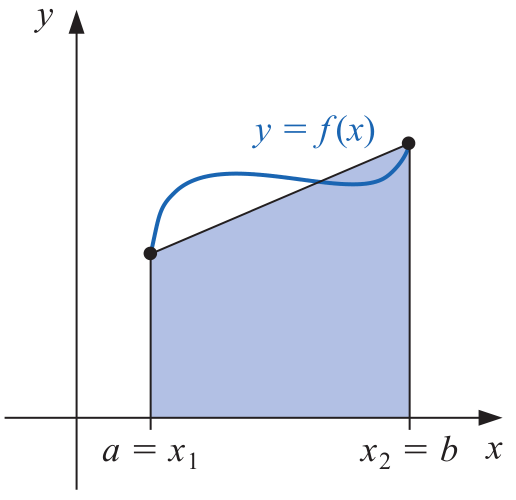
\includegraphics[width=.45\columnwidth]{./fig/Trapezoidal_rule.png}} \quad
\subfloat[Forest landscape.]{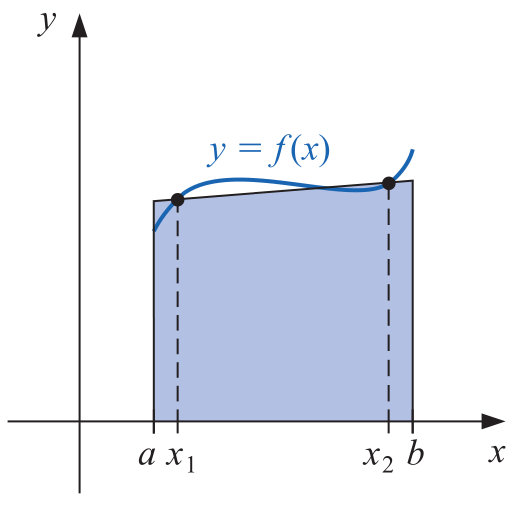
\includegraphics[width=.45\columnwidth]{./fig/Gaussian_quadrature.png}\label{fig:ComTraGau}}
\caption[Find optimal $C_i$ and $x_i$]{Find optimal $C_i$ and $x_i$.}%\caption[ ]
\end{figure}


\noindent Decision variables:\\
\begin{tabular}{lll}
 \quad$\left\{C_i\right\}$ &$i\in\left(1,n\right)$ & weights\\
 \quad$\left\{x_i\right\}$ &$i\in\left(1,n\right)$ & nodes
 \end{tabular}

\setcounter{equation}{0}
\noindent Objective
\begin{align*}
\min \quad
& \left|\int_{a}^{b}f(x)-\sum\limits_{i=1}^{n}c_if(x_i)\right|
\end{align*}

For every $f(x)$, polynomial and non-polynomial, $C_i$ and $x_i$ should achieve optimal. It is an open question now. To simply the question, we assume $f(x)$ is $P_n(x)$. Then the best choice of these values produces the exact
result for the largest class of polynomials, that is, the choice that gives the greatest degree
of precision.



\noindent Decision variables:\\
\begin{tabular}{lll}
 \quad$\left\{C_i\right\}$ &$i\in\left(1,n\right)$ & weights\\
 \quad$\left\{x_i\right\}$ &$i\in\left(1,n\right)$ & nodes
\end{tabular}

\setcounter{equation}{0}
\noindent Objective
\begin{align*}
\max  \quad
& degree(P(x)) \text{(measurement precision)}
\end{align*}
Constrains:\\
\begin{tabular}{l}
 \quad $P(x)$ is any polynomial whose degree is smaller than the given optimization goal.
\end{tabular}

\subsection{Proof}
Since $2n$ there are parameters to choose, $\max degree(P(x))=2n-1$. The method to find $C_i$ and $x_i$ is shown below.

\begin{defn}
The Laguerre polynomial $\{L_0(x),L_1(x)... \}$ is an orthogonal set on $\left[0,\infty\right)$ and satisfy $\int_0^\infty{e^{-x}L_i(x)L_j(x)dx=0}$, for $i \neq j$.
\end{defn}

\thm{Gaussian Laguerre rule}
Suppose that $x_1,x_2,...,x_n$ are the roots of the $n$th Laguerre polynomial $P_n(x)$ and that for each $i = 1,2,...,n$, the numbers $C_i$ are defined by \[
C_i=\int_{0}^{\infty}e^{-x}\prod\limits_{j=1,j\neq i}^{n}\frac{x-x_j}{x_i-x_j}dx
\]
if $P(x)$ is  any polynomial of degree less than $2n$, then
\[
\int_{0}^{\infty}{P(x)e^{-x}dx} = \sum\limits_{i=1}^{n}C_iP(x_i)
\]
which means the gaussian Laguerre rule has measurement of precision of $2n-1$
\\\textbf{proof}
Let us first consider the degree of  $P(x)$ is less than $ n$. Use Lagrange interpolation
\[
P(x) = \sum\limits_{i=1}^{n}P(x_i)L_i(x_i) + \frac{f^{(n+1)}(\xi(x))}{(n+1)!}\prod\limits_{i=1}^{n}(x-x_i)
\]
Since what we consider is just polynomial, we can see the error term is $0$. Then
\[
\int_{0}^{\infty}e^{-x}P(x)dx= \sum_{i=1}^{n}
{\left[
P(x_{i})\int_{0}^{\infty}e^{-x}\prod\limits_{
\begin{smallmatrix}
j =1 \\j\neq i
\end{smallmatrix}
}^{n}\frac{x-x_{j}}{x_{i}-x_{j}}dx
\right]
}
 = \sum\limits_{i=1}^{n}C_iP(x_i)
\]
Then, let us consider $P(x)$  ( $n \leq degree(P(x)) < 2n$ ). Divide $P(x)$ by the $n$th laguerre polynomial $P_n(x)$. Then we  get an R(x) as remainder. \[
P(x) = Q(x)P_n(x) + R(x).
\]
where $degree(Q(x)) < n$ and $ degree(R(x)) < n $.
According to the orthogonality  of laguerre polynomial,\[
\int_{0}^{\infty}e^{-x}P_n(x)Q(x)dx = 0
\]
Note that $x_i$ is a root of $P_n(x)$, so \[
P(x_i) = Q(x_i)P_n(x_i) + R(x_i) = R(x_i)
\]
Here $degree(R(x)) < n $, and fall into the case one, so
\[
\int_{0}^{\infty}e^{-x}R_n(x) = \sum\limits_{i=1}^{n}C_i R(x_i) = \sum\limits_{i=1}^{n}C_i P(x_i)
\]
Putting these facts together verifies that the formula is exact for the polynomial $P(x)$
\[
\int_{0}^{\infty}e^{-x}P(x)dx = \sum\limits_{i=1}^{n}C_i P(x_i)
\]


\subsection{Implement and Application}
The flow chart of my algorithm is shown in ~\vref{fig:flowchart}
\begin{figure}[tb]
\centering
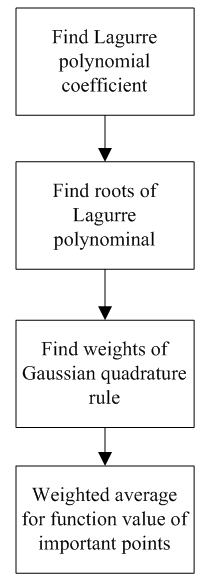
\includegraphics[width=.2\columnwidth]{./fig/flow_chart.png}
\caption[flow chart]{flow chart}
\label{fig:flowchart}

\end{figure}
My focus is implementing the quadrature rather than roots\_finding, the algorithm {\bf{Main2(symbolic\_compute).m}} implemented by myself will be shown below. And the file {\bf{Main1(use GUN).m}} uses the code distributed under the GNU LGPL license. (
\url{http://people.sc.fsu.edu/~jburkardt/m_src/gen_laguerre_rule/gen_laguerre_rule.html })
\lstinputlisting{../mcode/Main2_symbolic_compute.m}
First, let us see a successful example ~\vref{fig:1chux}.
\begin{figure}[tb]
\centering
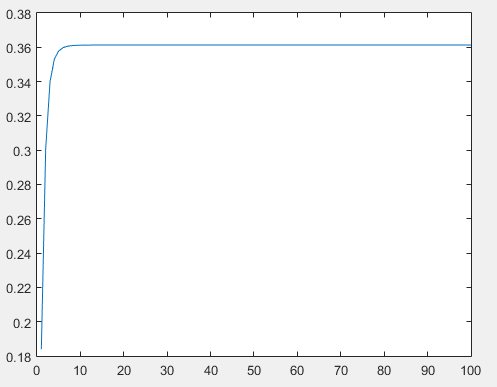
\includegraphics[width=.5\columnwidth]{./fig/1chux.png}
\caption[successful example]{successful example}
\label{fig:1chux}

\end{figure}
 We can see for \[
\int_{0}^{\infty}e^{-x}\frac{1}{1+x}dx
\]The result is the same as symbolic computation in matlab. And the rate of convergence is acceptable. It converges when degree of  Laguerre poly $n=5$.
But there are some problem occurred in the progress of integrating in the following.  \[\int_{0}^{\infty}e^{-x}\frac{1}{1+x}dx\] where $k=1.029811723741436e+07$, it converges and  computes slowly, refer to ~\vref{fig:Gauss_Laguerre}.
 \begin{figure}[tb]
\centering
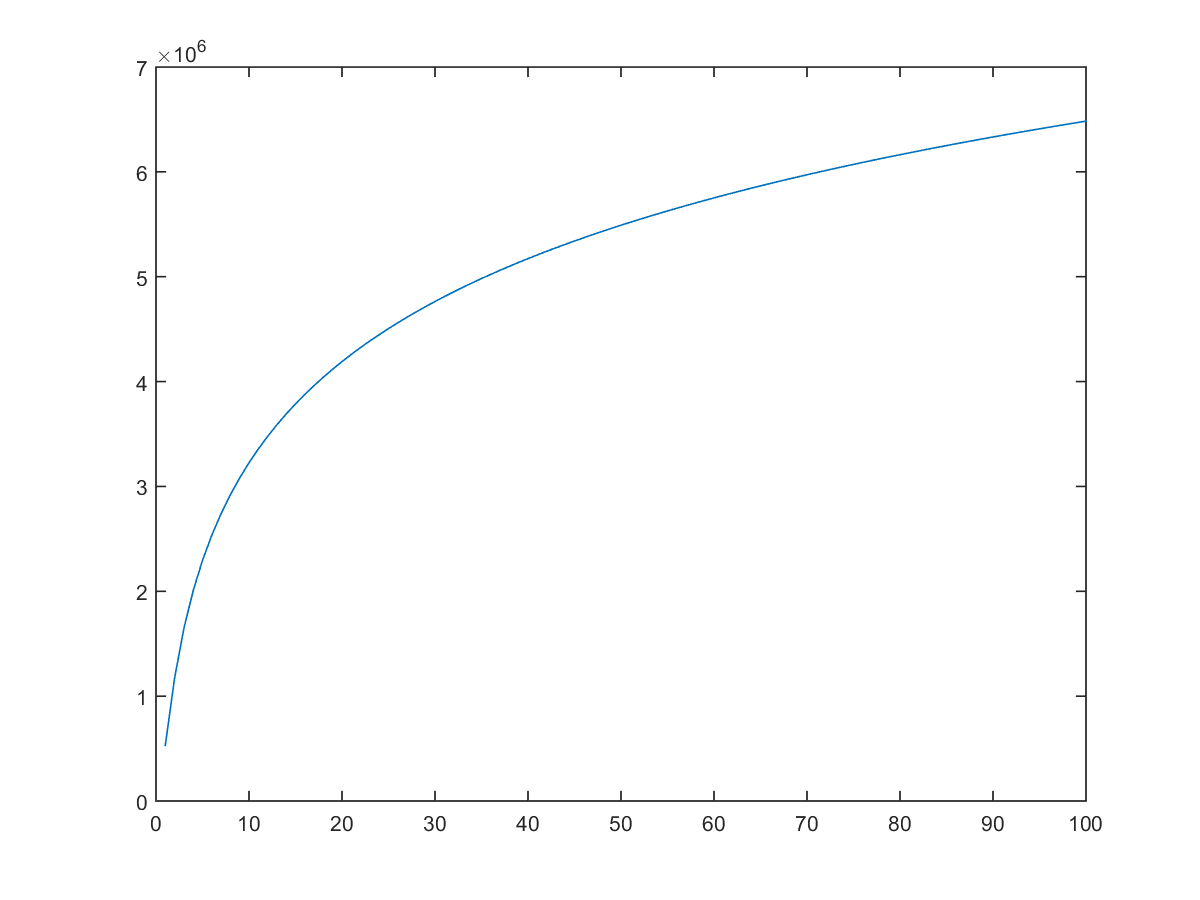
\includegraphics[width=.5\columnwidth]{./fig/Gauss_Laguerre.png}
\caption[Gauss\_Laguerre fail]{Gauss\_Laguerre fail}
\label{fig:Gauss_Laguerre}\end{figure}
Only when $n = 10000$, I get $2.179759274595623e+07
$, relatively close to $ 2.246313340780598e+07$ computed by symbolic tool,
and the time costed as high as $ b$ refer to ~\vref{fig:runtime}
\begin{figure}[tb]
\centering
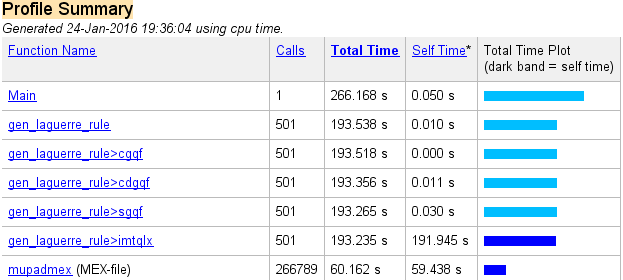
\includegraphics[width=.5\columnwidth]{./fig/runtime.png}
\caption[runtime]{runtime}
\label{fig:runtime}\end{figure}

I guess it is because $k$ is too big, so I have made many substitution and transforation first.
\begin{lstlisting}
[wi,xi,~]=gen_laguerre_rule(50,0,0,1);
double(k1*k*sum(wi.*subs(1/(1+k*x),x,xi)))
\end{lstlisting}

\begin{lstlisting}
[wi,xi,~]=gen_laguerre_rule(50,0,0,1/k);
double(k1*sum(wi.*subs(1/(1+x),x,xi)))
\end{lstlisting}

\begin{lstlisting}
double(int(exp(-x)/x,x,1/k,inf)*exp(1/k)/k*k*k1)
[wi,xi,~]=gen_laguerre_rule(50,0,1/k,1);
double(exp(1/k)/k*k*k1*sum(wi.*subs(1/x,x,xi)))
\end{lstlisting}
Then I try to implement all algorithm  via symbol computation, which means immense accuracy, but the time-consuming is great and I only wait for the result $2.138289534346160e+07$

\subsection{Analysis}
It is apparently this algorithm will converge slowly if $n$ is huge, but why it suffers  big error when $n$ is small? We can illustrate it by ~\vref{fig:Runge}.
When $k$ is quite huge the influence of Runge\'s phenomenon will be amplified.
\\To sum up, Gaussian quadrature as above will only produce accurate results if the function $f(x)$ is well approximated by a polynomial function within the range $\left(0, \infty\right]$.
\\Finally, I guess  there are still many other objective function and may result other methods to improve its performance.\\
\begin{centering}
\begin{tabular}{ll}
\hline
strength&weakness\\
\hline
\begin{tabular}{l}
 Accurate when condition is satisfied\\
\end{tabular}
&
\begin{tabular}{l}
  % after \\: \hline or \cline{col1-col2} \cline{col3-col4} ...
  Invoking f(x) be well approximated\\
   by a polynomial function\\

\end{tabular}
   \\
\hline
\begin{tabular}{l}
  % after \\: \hline or \cline{col1-col2} \cline{col3-col4} ...
  Tabular for laguerre ploy can be\\
  made previously \\
\end{tabular}

&

\begin{tabular}{l}
  % after \\: \hline or \cline{col1-col2} \cline{col3-col4} ...
  Accurate when f(x) is polynomial,\\
  and I can not decided \\
    the accuracy for f(x) in other form.\\
\end{tabular}


\\
\hline
&
\begin{tabular}{l}
  % after \\: \hline or \cline{col1-col2} \cline{col3-col4} ...
  Without error bound.\\
\end{tabular}
\\
\hline

&\begin{tabular}{l}
  % after \\: \hline or \cline{col1-col2} \cline{col3-col4} ...
  Cannot use composite method \\ to be more accuracy.\\
\end{tabular}\\
\hline
\end{tabular}
\end{centering}


\begin{figure}[tb]
\centering
\subfloat[degree=3]{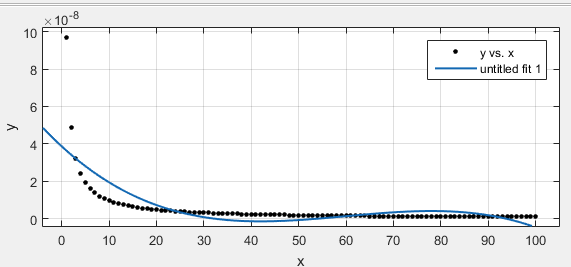
\includegraphics[width=.45\columnwidth]{./fig/lg3.png}} \quad
\subfloat[degree=7]{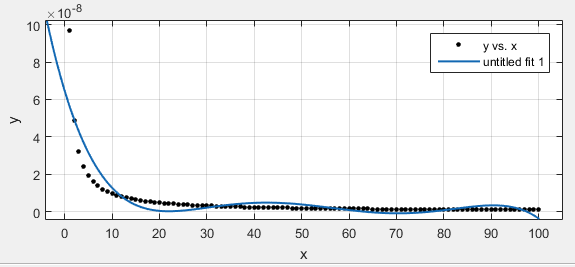
\includegraphics[width=.45\columnwidth]{./fig/lg2.png}\label{fig:Runge}} \\
\subfloat[degree=13]{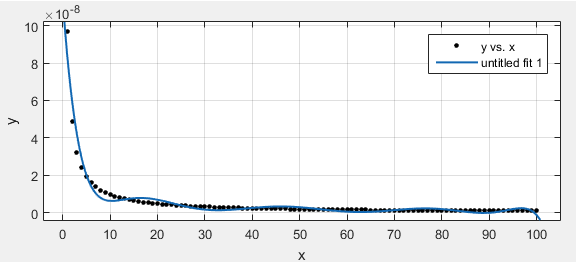
\includegraphics[width=.45\columnwidth]{./fig/lg1.png}} \quad
\caption[Runge\'s phenomenon]{Runge\'s phenomenon} % The text in the square bracket is the caption for the list of figures while the text in the curly brackets is the figure caption
\label{fig:esempio}
\end{figure}

\section{adaptive quad}
Since Gauss Laguerre method on the book is not suitable for this question, I must quest for more accurate and fast method.
\subsection{Infinite to Finite}
A one-parameter family of transformations can be made by splitting the range $\left[0,\infty \right)$ into two intervals $\left[0,S\right]$ and $\left[S, \infty \right)$. And apply $t=x/S$, we get
\begin{align}
 \int_{0} ^{\infty}f(x)dx =& \int_{0} ^{\infty}\frac{e^{-x}}{1+kx}dx  \\
=& S \int _{0} ^{1} [f(St)+t^{-2}f(S/t)]dt\\
=& S{\mkern 1mu} \int_0^1 {\left( {\frac{{{{\rm{e}}^{ - S{\kern 1pt} t}}}}{{kS{\mkern 1mu} t + 1}} + \frac{{{{\rm{e}}^{ - \frac{S}{t}}}}}{{t{\mkern 1mu} \left( {kS + t} \right)}}} \right)} dt\\
=&def \, as = S \int _{0} ^{1} (f_1(x)+f_2(x))dx
\end{align}
\subsection{Why choose it?}
Observe $f(x), f_1(x),f_2(x)$, (refer to ~\vref{fig:Observation}) $f_2(x) $ change rapidly in a very small range, $f_x(s)$ contain its function value mainly on a range very close to 0. Thus, $f_1(x)$ is the main parts of integration. To sum up,
\begin{itemize}
  \item We should not abandon $f_2(x)$ for accuracy purpose. The sensitivity of $S$ should be checked.
  \item Why Romberg or other  Newton-Cotes formulas which use values of the function at equally-spaced points fail. Because they can not focus on the small region, wasting time on trivial things?
  \item Why Gaussian Laguerre fail? Because it cannot divided and conquer, cannot iterate from last result to a more accurate result.
\end{itemize}

\begin{figure}[tb]
\centering
\subfloat[$f(x)$]{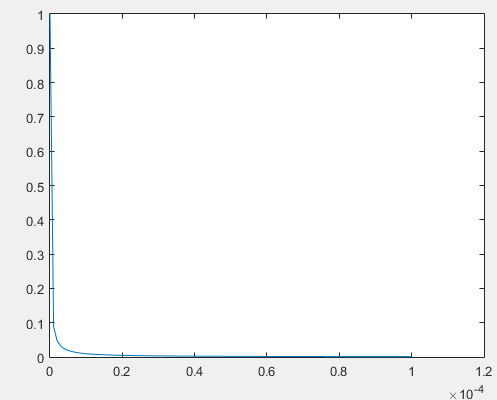
\includegraphics[width=.45\columnwidth]{./fig/f.png}} \quad
\subfloat[$f_2(x)$]{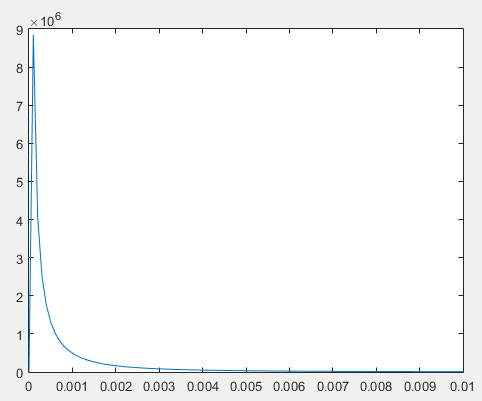
\includegraphics[width=.45\columnwidth]{./fig/f1.png}} \\
\subfloat[$f_1(x)$]{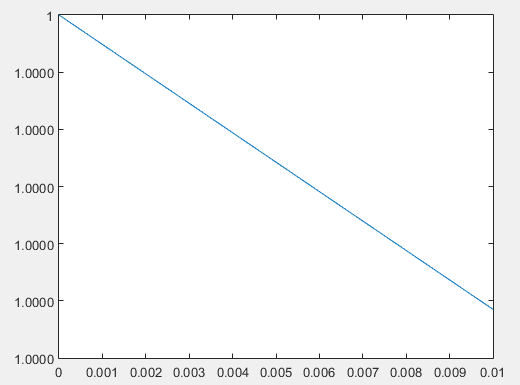
\includegraphics[width=.45\columnwidth]{./fig/f2.png}\label{fig:Observation}}

\caption[Change rapidly]{Change rapidly} % The text in the square bracket is the caption for the list of figures while the text in the curly brackets is the figure caption
\end{figure}

\subsection{Implement and Results}
A rather accurate results $2.246313340780605e+07
$ compared to $ 2.246313340780598e+07$ with relative error of $ 3.150963598256511e-15$ can be resulted quite fast in just $7.111s$ when $S=0.0001$
\lstinputlisting{../mcode/adapt_simp.m}
\subsection{Sensitivity of S}
Refer to ~\vref{fig:sense}, we can see from 1 down to 0.00001 the results is more and more close to symbolic answer. Meanwhile ,the costs of time also increase. Overall, compared to its accuracy, this kind of slightly unstable is acceptable.
\begin{figure}[tb]
\centering
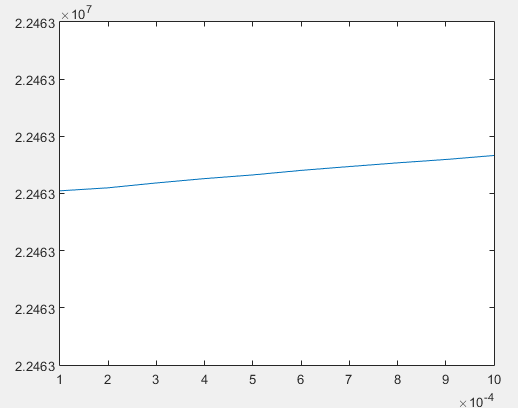
\includegraphics[width=.5\columnwidth]{./fig/sense.png} 


\caption[Sensitivity of S]{Sensitivity of S}
\label{fig:sense}

\end{figure}

\section*{Appendix}
Weights and nodes of Laguerre polynomial\\
\begin{centering}
\begin{tabular}{lll}
\hline
i &xi &wi \\
\hline
1&3.570039E-02&8.841211E-02\\
\hline
2&1.881623E-01&1.768147E-01\\
\hline
3&4.626943E-01&2.113631E-01\\
\hline
4&8.597730E-01&1.940812E-01\\
\hline
5&1.380011E+00&1.464343E-01\\
\hline
6&2.024209E+00&9.332680E-02\\
\hline
7&2.793369E+00&5.093220E-02\\
\hline
8&3.688703E+00&2.397619E-02\\
\hline
9&4.711641E+00&9.774625E-03\\
\hline
10&5.863851E+00&3.457940E-03\\
\hline
11&7.147248E+00&1.062247E-03\\
\hline
12&8.564017E+00&2.832717E-04\\
\hline
13&1.011663E+01&6.550941E-05\\
\hline
14&1.180789E+01&1.311607E-05\\
\hline
15&1.364093E+01&2.268453E-06\\
\hline
16&1.561929E+01&3.379626E-07\\
\hline
17&1.774691E+01&4.322821E-08\\
\hline
18&2.002823E+01&4.728494E-09\\
\hline
19&2.246825E+01&4.403174E-10\\
\hline
20&2.507256E+01&3.472441E-11\\
\hline
21&2.784748E+01&2.305382E-12\\
\hline
22&3.080015E+01&1.279773E-13\\
\hline
23&3.393866E+01&5.894177E-15\\
\hline
24&3.727225E+01&2.232218E-16\\
\hline
25&4.081149E+01&6.880336E-18\\
\hline
26&4.456860E+01&1.705604E-19\\
\hline
27&4.855776E+01&3.353712E-21\\
\hline
28&5.279561E+01&5.146200E-23\\
\hline
29&5.730186E+01&6.044763E-25\\
\hline
30&6.210018E+01&5.310585E-27\\
\hline
31&6.721937E+01&3.392528E-29\\
\hline
32&7.269516E+01&1.521735E-31\\
\hline
33&7.857280E+01&4.585292E-34\\
\hline
34&8.491123E+01&8.762159E-37\\
\hline
35&9.178987E+01&9.827416E-40\\
\hline
36&9.932081E+01&5.801152E-43\\
\hline
37&1.076724E+02&1.530909E-46\\
\hline
38&1.171223E+02&1.381986E-50\\
\hline
39&1.282018E+02&2.566634E-55\\
\hline
40&1.422800E+02&2.700361E-61\\
\hline
\end{tabular}
\end{centering}

\lstinputlisting{../mcode/Main1_use_GUN.m}
\lstinputlisting{../mcode/Main3_simpson_adp.m}

\end{document}
